%!TEX root = ../calculus_tutorial.tex

\section*{Overview and a look ahead}

	The goal of this tutorial is to introduce you to the language of calculus.
	The concept map in Figure~\ref{fig:calculus_tutorial_overview}
	shows an overview of the calculus ideas you'll learn in the next few pages.

	\begin{figure}[htb]
		\centering
		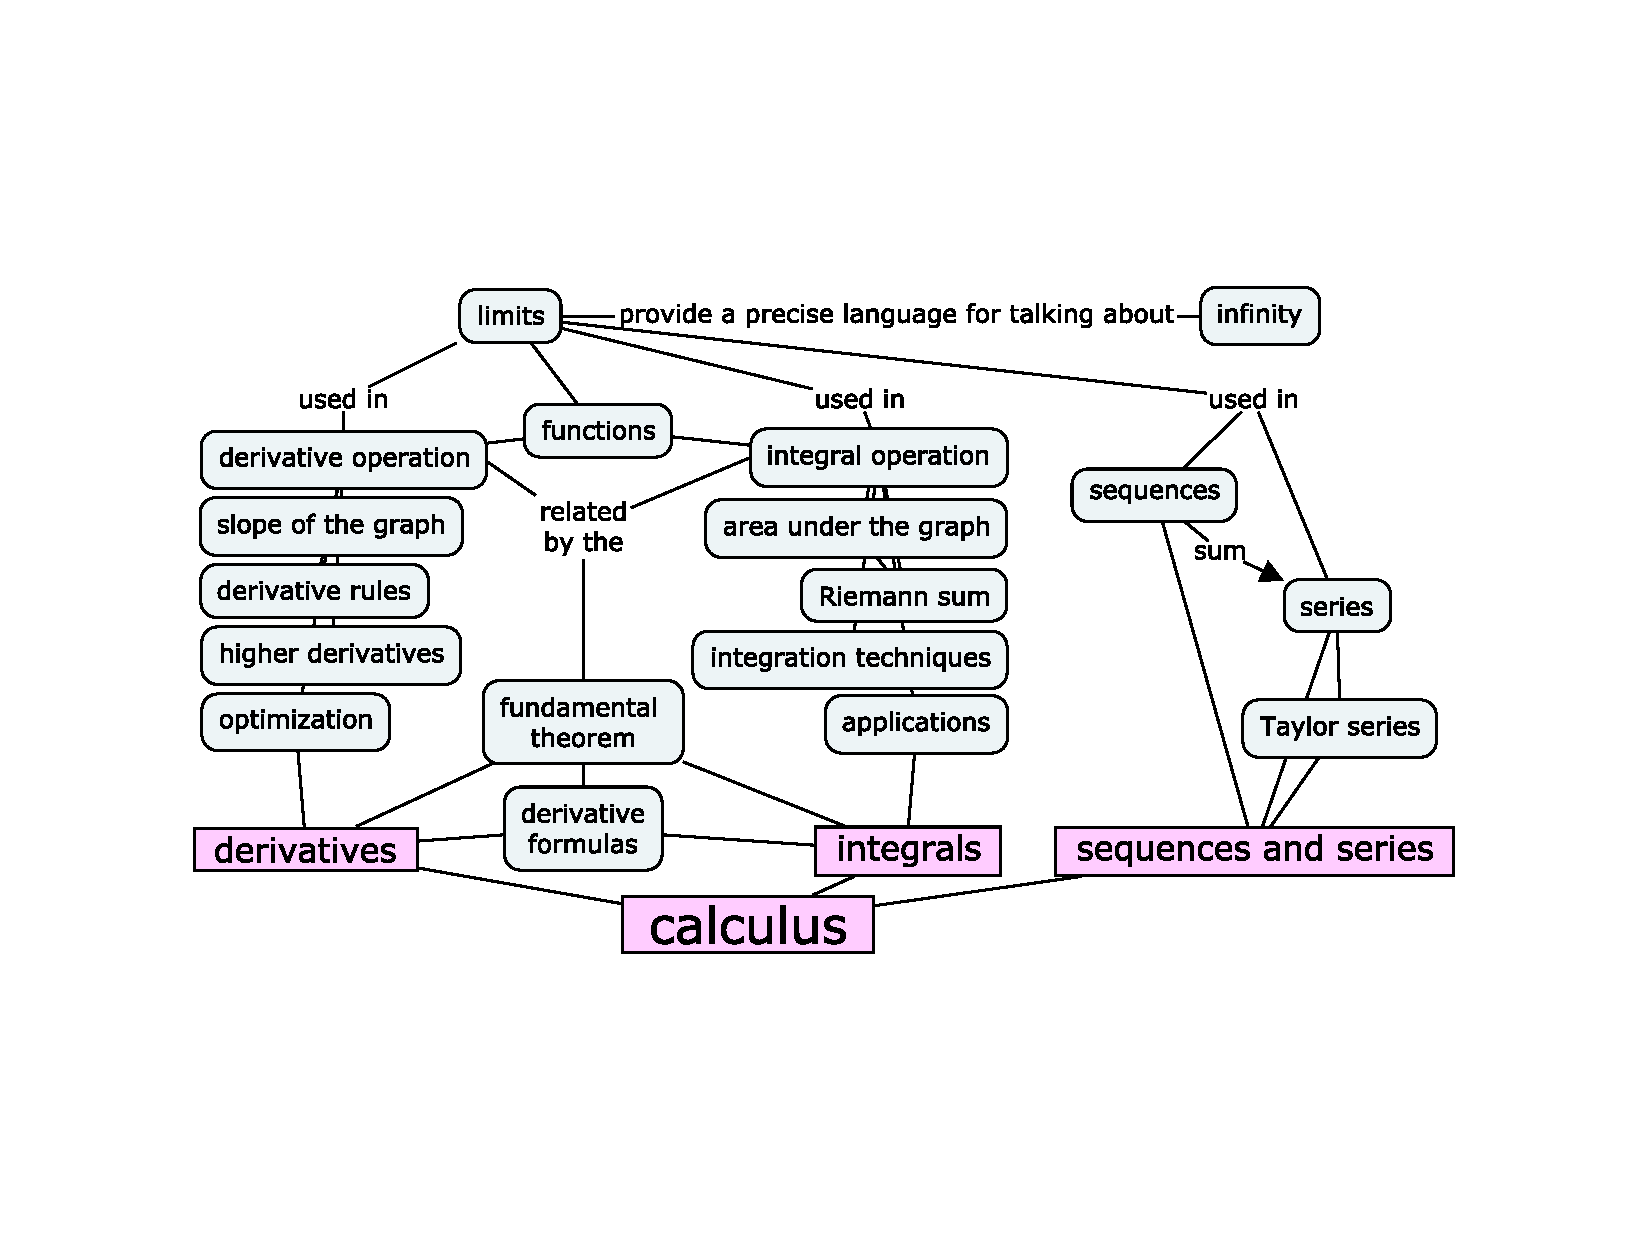
\includegraphics[width=0.99\columnwidth]{figures/calculus/calculus_tutorial_overview.pdf}%
		\vspace{-2mm}
		\caption{	The calculus concepts and topics you'll learn in this tutorial.}
		\label{fig:calculus_tutorial_overview}
	\end{figure}

	We'll start % theis tutorial
	by introducing limits in Section~\ref{sec:limits}.
	Limits give us a precise language to talk about infinity.
	% ALT: talk about infinitely large and infinitely small quantities
	Limits are a cornerstone idea in calculus,
	because they allow us to define the calculus operations:
	derivatives, integrals, and series.
	%
	We'll discuss derivatives 
	in Section~\ref{sec:derivatives}
	and integrals in Section~\ref{sec:integrals}.
	We'll then talk about sequences and series
	in Section~\ref{sec:sequences_and_series},
	and conclude with a brief intro to multivariable calculus in Section~\ref{sec:multivariable_calculus}.

	Throughout the tutorial,
	we'll explain concepts using text, formulas, graphs, and code examples.
	My intention is for you to understand the key ideas of calculus in theory,
	but also learn practical skills you can use to solve real-world problems.

